% section 3
% Kota Miura (miura@embl.de)

\section{Filtering}

Filtering improves the appearance of digital image. Then recognition of
shapes becomes easier by noise removing and enhancement of the
structural edge. Not only for the appearance, filtering improve the
efficiency of "segmentation" which we
will study in the next section. Segmented image could be used as a mask
to specify regions to be measured. Note that the filtering alters the
image so one must realize that in most cases, processed images cannot
be used for quantitative intensity measurement without precise
knowledge on what would happen to the numerical values after the
processing. 

There are two different types of filtering: one involves the frequency
domain of images (Fourier transformed image), while the others deals
with spatial domain. We first study the spatial domain filtering and
its central concept "convolution", and
walk through various types of convolutions. We then study the frequency
domain filtering (FFT). In FFT world, convolution of an image with
filter kernel could be done simply by multiplication between two
images. 



\subsection{Convolution }

In the \ijmenu{[Process]} menu, we see a long list of
filters. An important concept for understanding what these commands
will do to your image is "convolution".
A small mask (called kernel) is moved along the image pixel by pixel
and apply operations using the surrounding pixel values (see Fig.
\ref{fig:img38}). The result of operation is over-written to that pixel position
as the new pixel value.


%figure
\begin{figure}[htbp]
\begin{center}
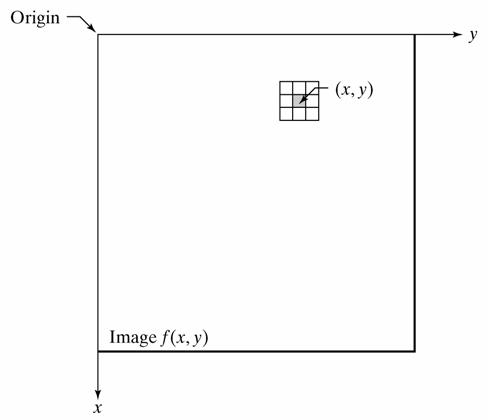
\includegraphics[width=7cm]{img/CMCIBasicCourse201102-img38.png}
\caption{ An image and a Kernel (figure taken from DIP)}
\label{fig:img38}
\end{center}
\end{figure}


To understand how the convolution is done, we take a one-dimensional
example (Fig. \ref{fig:img39}).


%figure
\begin{figure}[htbp]
\begin{center}
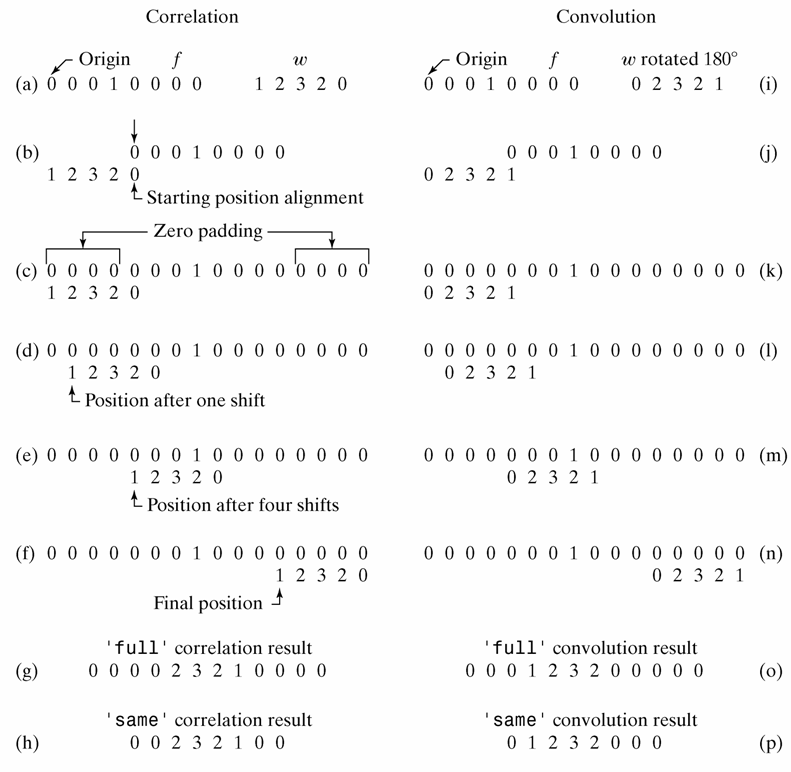
\includegraphics[width=11.718cm]{img/CMCIBasicCourse201102-img39.png}
\caption{ 1-dimensional convolution and correlation (figure taken from DIP)}
\label{fig:img39}
\end{center}
\end{figure}

We have a small 1D array $f$, and we want to convolve this with a
kernel $w$ (i). We first rotate the kernel by 180 degrees that
the order is now reversed. Then we align $f$ and $w$ to
match the position of the last element of kernel to the first element
of $f$. Since we want to have all the kernel elements to have
corresponding partner, we "pad" $f$ by 0.
This is just for the convenience of calculation (k). Then you multiply
each element pairs (5 pairs in this case) and sum up the results. since
all partners in $f$ are 0, the sum of multiplication is 0. We note this
as the first element of "full convolution
result" (o). We then slide $w$ to the left by one
element, do the multiplications and summing up again. Note the result
as the second element of "full convolution
result" (o). Like wise, we do such calculation step by
step until last element of $w$ matches the last element of
$f$ (n). After then, we throw away padded elements from the
output 1D array to have a resulting array with same length as the
original $f$ (p). 

%{\selectlanguage{english}\sffamily

\begin{quote}
{\sffamily\bfseries
Convolution and correlation}

Two closely-related bilinear operations that are especially important
for information processing are $convolution$ and
$correlation$. In the simplest case, correlation can
be described as a comparison of two fields at all possible relative
positions. More specifically, if $\chi$
is the correlation of two one-dimensional fields $\phi$
and $\psi$, $\chi = \phi*\psi$, then $\chi(r)$ reflects how well 
$\phi$ and $\psi$ match (in an inner-product sense) when relatively displaced by
$r$. Mathematically, 
\[
\chi(r)=\int_{\Omega }^{} \phi(s-r)\psi (s)ds
\]
Higher dimensional correlations are the same, except that $r$ is
a relative displacement $vector$ rather than a scalar. 

$Convolution$, $\chi=\phi\otimes \psi$, is essentially the same as correlation, except that the field $\phi$ is reflected before the comparison takes place: 
\[
\chi(r)=\int_{\Omega }^{}  \phi(r-s)\psi  (s)ds
\]
Convolution is useful because: (1) its algebraic properties are more
like multiplication, and thus more familiar, than correlation; and (2)
many physical processes (e.g. linear systems, such as dendritic nets)
perform convolutions.

%Two closely-related bilinear operations that are especially important
%for information processing are \textit{convolution} and
%\textit{correlation}. In the simplest case, correlation can
%be described as a comparison of two fields at all possible relative
%positions. More specifically, if 
%
\includegraphics[width=0.185cm,height=0.344cm]{img/CMCIBasicCourse201102-img40.png}
%is the correlation of two one-dimensional fields 
%
\includegraphics[width=0.212cm,height=0.503cm]{img/CMCIBasicCourse201102-img41.png}
%and 
%
\includegraphics[width=0.212cm,height=0.503cm]{img/CMCIBasicCourse201102-img42.png}
%, 
%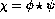
\includegraphics[width=1.455cm,height=0.503cm]{img/CMCIBasicCourse201102-img43.png}
%, then 
%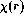
\includegraphics[width=0.635cm,height=0.556cm]{img/CMCIBasicCourse201102-img44.png}
%reflects how well 
%
\includegraphics[width=0.212cm,height=0.503cm]{img/CMCIBasicCourse201102-img45.png}
%and 
%
\includegraphics[width=0.212cm,height=0.503cm]{img/CMCIBasicCourse201102-img46.png}
%match (in an inner-product sense) when relatively displaced by
%\textit{r}.\href{http://www.cs.utk.edu/~mclennan/anon-ftp/FCMC-tr/footnode.html#516}{
%
\includegraphics[width=0.397cm,height=0.397cm]{img/CMCIBasicCourse201102-img47.png}
%}
% Mathematically, 
%
%
\includegraphics[width=13.227cm,height=0.716cm]{img/CMCIBasicCourse201102-img48.png}
%
%Higher dimensional correlations are the same, except that \textit{r} is
%a relative displacement \textit{vector} rather than a
%scalar. 
%
%\textit{Convolution}, 
%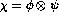
\includegraphics[width=1.561cm,height=0.503cm]{img/CMCIBasicCourse201102-img49.png}
%, is essentially the same as correlation, except that the field 
%
\includegraphics[width=0.212cm,height=0.503cm]{img/CMCIBasicCourse201102-img50.png}
%is reflected before the comparison takes place: 
%
%
\includegraphics[width=13.227cm,height=0.716cm]{img/CMCIBasicCourse201102-img51.png}
%
%Convolution is useful because: (1) its algebraic properties are more
%like multiplication, and thus more familiar, than correlation; and (2)
%many physical processes (e.g. linear systems, such as dendritic nets)
%perform convolutions.


Quote from:
\url{http://www.cs.utk.edu/\~mclennan/anon-ftp/FCMC-tr/node14.html}
\end{quote} 

In two dimensional matrix, see the example in Fig. \ref{fig:img52}. 

%figure
\begin{figure}[htbp]
\begin{center}
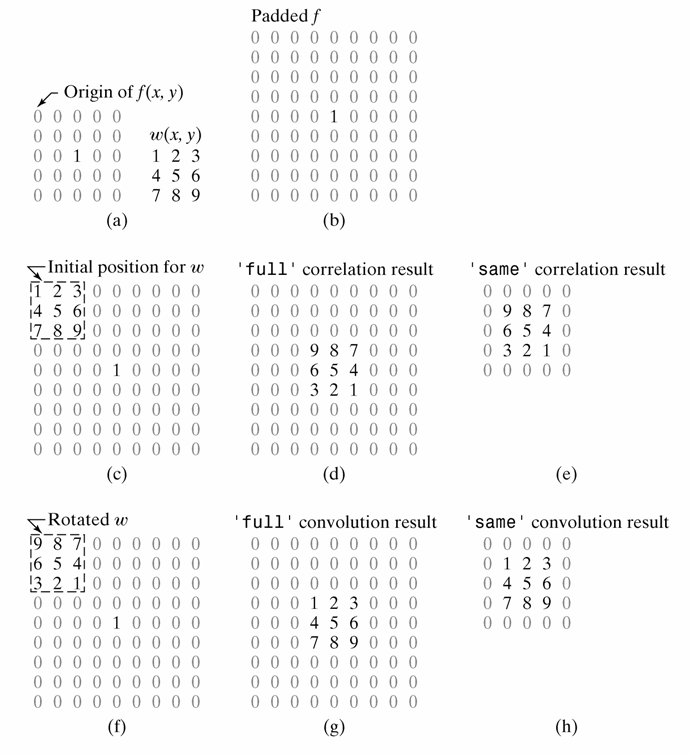
\includegraphics[width=10cm]{img/CMCIBasicCourse201102-img52.png}
\caption{ Two-dimensional convolution (figure taken from DIP)}
\label{fig:img52}
\end{center}
\end{figure}

The matrix (a) is first padded (b), then starting from the top-left
corner (f) the matrix is convoluted (g) and then the padded rows and
columns are removed to return an output matrix with the same dimension
as the original (h).

\subsection{Kernels}

In \ijmenu{[Process]} menu, we have many operators such
as smooth, sharpen, find edges\dots and so on. Many of them ate
called "linear filters" because
the result of filtering is a linear combination of the original image
pixel values. We study various kernels in this section. 

\subsubsection{Smoothening}
\ "Smoothening" operation, which is
used for attenuating noise (Median kernel is better for shot-noise
removal but for learning purpose we stick to the smoothing), is done by
applying the following kernel to the image. 

%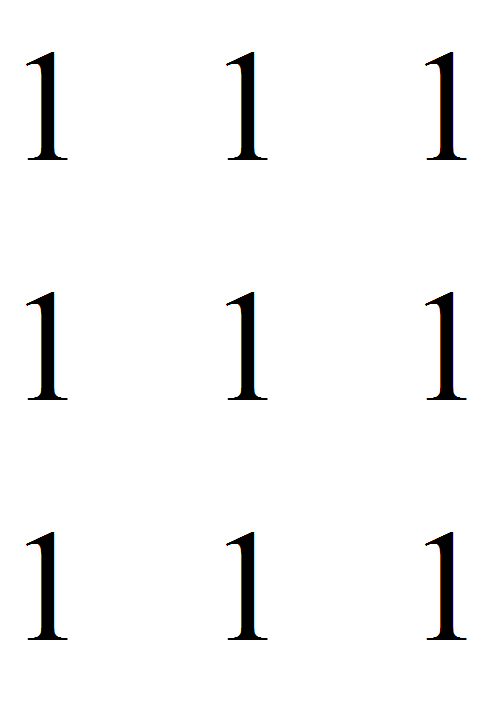
\includegraphics[width=1.305cm,height=1.87cm]{img/CMCIBasicCourse201102-img53.png}
\[
 \begin{matrix}
  1 & 1 & 1 \\
  1 & 1 & 1 \\
  1 & 1 & 1
 \end{matrix}
\]

Let"s take an example of an image with a vertical line
in the middle.


\[
 \begin{matrix}
  0 & 0 & 10 & 0 & 0 \\
  0 & 0 & 10 & 0 & 0 \\
  0 & 0 & 10 & 0 & 0 \\
  0 & 0 & 10 & 0 & 0 \\
  0 & 0 & 10 & 0 & 0 
 \end{matrix}
\]

%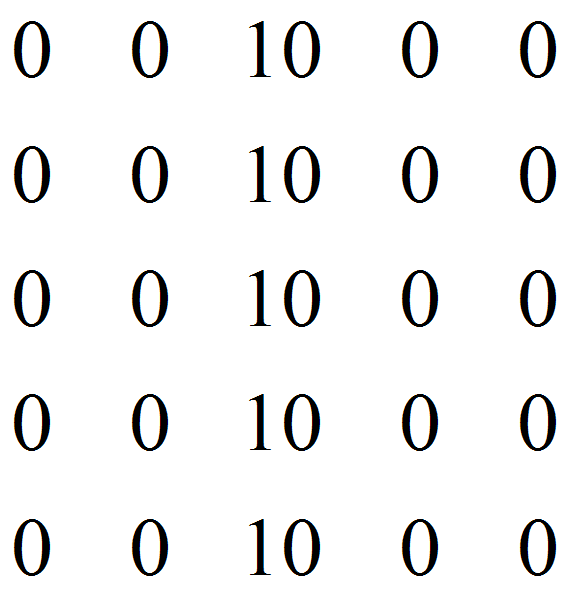
\includegraphics[width=2.928cm,height=3.104cm]{img/CMCIBasicCourse201102-img54.png}

Just for now, we forget about the padding for explanation, and first
apply the kernel to the top-left corner for
calculating convolved value at (1, 1) pixel position (note: top-left element position is (0, 0)).
Then the calculation is


$output( 1 , 1 )$\\
$\quad = ( 0 \times 1 + 0 \times 1 + 0 \times 1 + $\\
$\qquad 0 \times 1 + 0 \times 1 + 0 \times 1 + $\\
$\qquad 10 \times 1 + 10 \times 1 + 10 \times 1 ) / 9 $\\
$\quad = 30 / 9 $\\
$\quad = 3$

The sum of multiplication is divided by 9, which is the sum of all
elements in the kernel. This is to normalize the convolution, so that
the output value will not to be too large compared to the original. We
then shift the kernel one step in x-direction, and apply the kernel for
calculating (2, 1) position. 

$output( 2 , 1)$\\
$\quad = ( 0 \times 1 + 0 \times 1 + 0 \times 1 + $\\
$\qquad 10 \times 1 + 10 \times 1+ 10 \times 1 +$\\ 
$\qquad 0 \times 1 + 0 \times 1 + 0 \times 1) / 9 $\\
$\quad = 30 / 9$\\ 
$\quad = 3$

You might have now understood that the
"smooth" operation is actually
averaging the values in the surrounding. Applying the kernel through
the image, the new image will be: 

%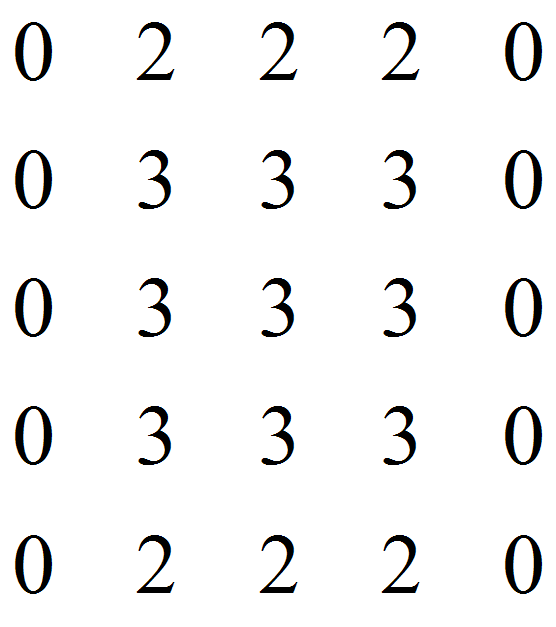
\includegraphics[width=2.752cm,height=3.104cm]{img/CMCIBasicCourse201102-img55.png}

\[
 \begin{matrix}
  0 & 2 & 2 & 2 & 0 \\
  0 & 3 & 3 & 3 & 0 \\
  0 & 3 & 3 & 3 & 0 \\
  0 & 3 & 3 & 3 & 0 \\
  0 & 2 & 2 & 2 & 0 
 \end{matrix}
\]
The vertical line is then now broader and darker -- the smoothing
effect. Note that the pixels in the first and the 5th rows were
calculated with zero padding so that values are 2 rather than 3. This
is the boundary effect unavoidable with any filtering by convolution.
We could attenuate this effect if we do padding by duplicating
neighboring pixels. Then the result of convolution then becomes

%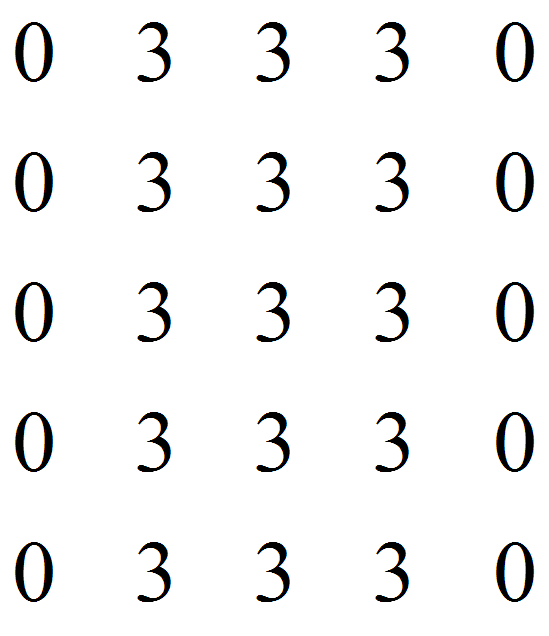
\includegraphics[width=2.681cm,height=3.104cm]{img/CMCIBasicCourse201102-img56.png}
\[
 \begin{matrix}
  0 & 3 & 3 & 3 & 0 \\
  0 & 3 & 3 & 3 & 0 \\
  0 & 3 & 3 & 3 & 0 \\
  0 & 3 & 3 & 3 & 0 \\
  0 & 3 & 3 & 3 & 0 
 \end{matrix}
\]

\begin{indentexercise}{1}
 Working with kernel: in ImageJ, one could
design original kernel and do convolution for images.
Open \textbf{microtubule.tif} image and
zoom up so you can see individual pixels. Do \ijmenu{[Process
> Filter > Convolve]}. A pop-up window
appears (see the image below). One could edit the kernel. Be sure to
make spaces between numbers. By clicking OK, the kernel will be applied
to the image. 

Try replacing the default kernel with the smoothening kernel we studied
above. Apply the kernel to sample image
\textbf{microtubule.tif}. Increase the
dimension to 5 x 5, 9 x 9 and do the smoothening. 

\textbf{Question}: what happened when the size of the kernel became
larger? Check the preview option, so that the change in the kernel
could be visualized directly while editing.

%figure
\begin{figure}[htbp]
\begin{center}
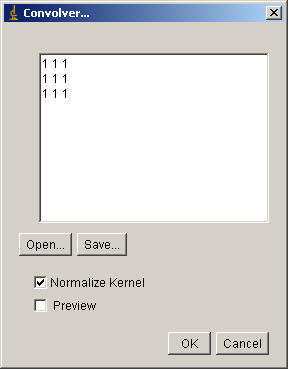
\includegraphics[width=4.471cm]{img/CMCIBasicCourse201102-img57.png}
\caption{ Convolver Window.}
\label{fig:img57}
\end{center}
\end{figure} 

\end{indentexercise}

\subsubsection{Sharpen }

%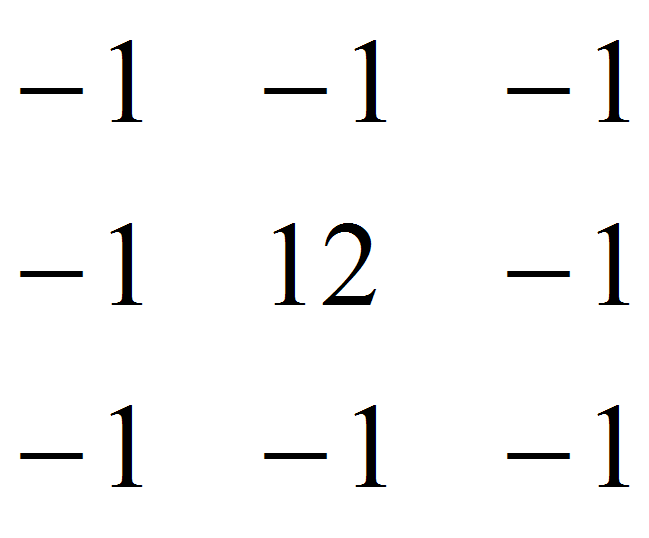
\includegraphics[width=2.258cm,height=1.87cm]{img/CMCIBasicCourse201102-img58.png}
\[
 \begin{matrix}
  -1 & -1 & -1 \\
  -1 & 12 & -1 \\
  -1 & -1 & -1
 \end{matrix}
\]

This kernel sharpens the image, also known as Laplacian. Side effect:
noise is also enhanced. 


\subsubsection{Find Edge (gradient)}
\label{subsub:findedgekernel}
Following two kernels are applied independently. Square root of the sum
of the square of two result images will be calculated (called
"Sobel Filter": for more details,
see Appendix \ref{app3}) \ 

%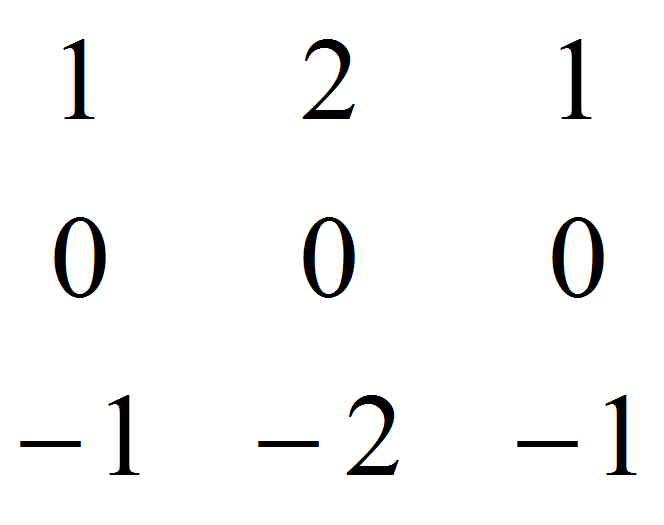
\includegraphics[width=2.364cm,height=1.87cm]{img/CMCIBasicCourse201102-img59.png}
\[
 \begin{matrix}
  1 & 2 & 1 \\
  0 & 0 & 0 \\
  -1 & -2 & -1
 \end{matrix}
\]
and

%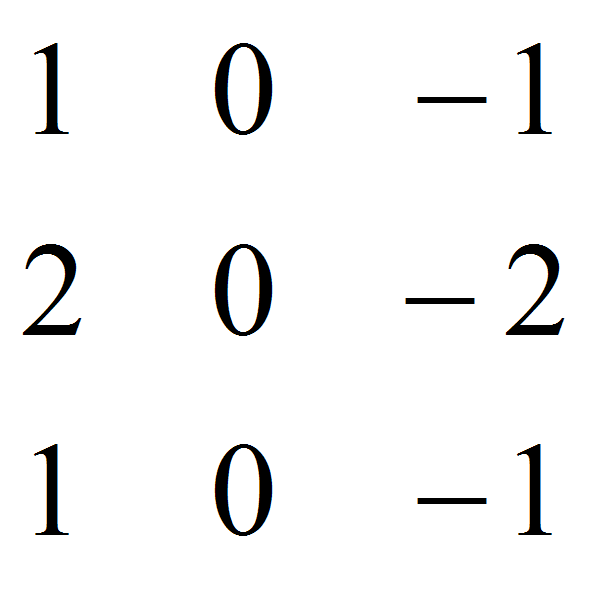
\includegraphics[width=1.87cm,height=1.87cm]{img/CMCIBasicCourse201102-img60.png}
\[
 \begin{matrix}
  1 & 0 & -1 \\
  2 & 0 & -2 \\
  1 & 0 & -1
 \end{matrix}
\]


\subsubsection{Gaussian Blur}

This kernel blurs (in positive sense, we call it
"smooth") the image by convolution
using a square Gaussian (bell-shaped) kernel. The width of the kernel,
in pixels, is 2*\textit{sigma}+1, where \textit{sigma} is entered into
a dialog box (ImageJ documentation). Following three kernels are with
different sigma 2 (5x5), 3 (7x7) and 7 (15x15). 

Gauss 5 x 5 (Sigma = 2)
 
%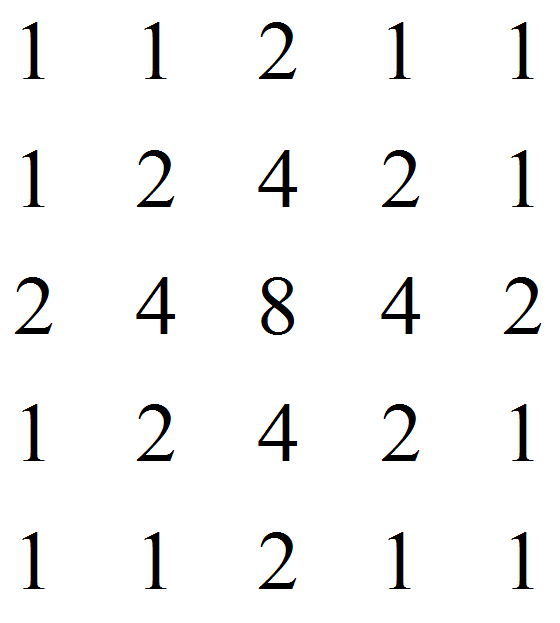
\includegraphics[width=2.785cm,height=3.104cm]{img/CMCIBasicCourse201102-img61.png}
\[
 \begin{matrix}
  1 & 1 & 2 & 1 & 1\\
  1 & 2 & 4 & 2 & 1\\
  2 & 4 & 8 & 4 & 2\\
  1 & 2 & 4 & 2 & 1\\
  1 & 1 & 2 & 1 & 1
 \end{matrix}
\]

Gauss 7 x 7 (Sigma = 3)

%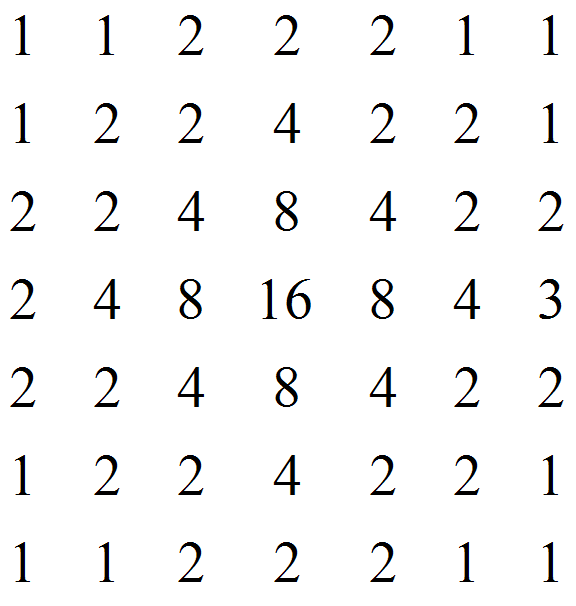
\includegraphics[width=4.163cm,height=4.374cm]{img/CMCIBasicCourse201102-img62.png}
\[
 \begin{matrix}
  1 & 1 & 1 & 2 & 1 & 1 & 1\\
  1 & 2 & 2 & 4 & 2 & 2 & 1\\
  2 & 2 & 4 & 8 & 4 & 2 & 2\\
  2 & 4 & 8 & 16 & 8 & 4 & 2\\
  2 & 2 & 4 & 8 & 4 & 2 & 2\\
  1 & 2 & 2 & 4 & 2 & 2 & 1\\
  1 & 1 & 1 & 2 & 1 & 1 & 1
 \end{matrix}
\]
Gauss 15 x 15 (Sigma = 7)

%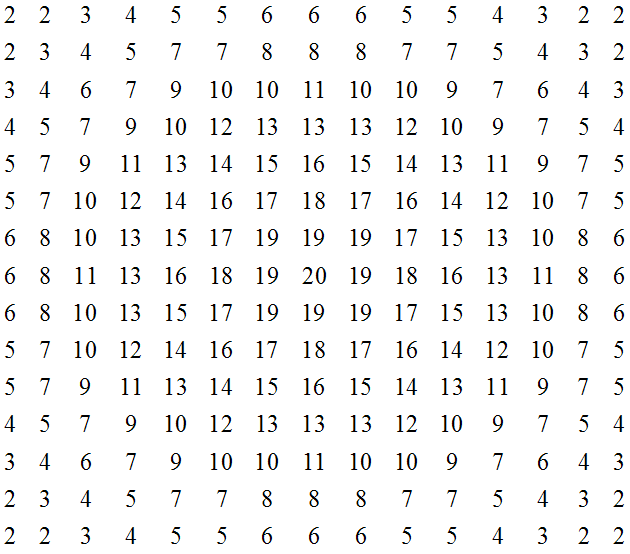
\includegraphics[width=10.76cm,height=9.454cm]{img/CMCIBasicCourse201102-img63.png}
% to make a large matrix, http://newsgroups.derkeiler.com/Archive/Comp/comp.text.tex/2008-07/msg00905.html
\setcounter{MaxMatrixCols}{16}
\[
\begin{matrix}
  2 & 2 & 3 & 4 & 5 & 5 & 6 & 6 & 6 & 5 & 5 & 4 & 3 & 2 & 2\\
  2 & 3 & 4 & 5 & 7 & 7 & 8 & 8 & 8 & 7 & 7 & 5 & 4 & 3 & 2\\
  3 & 4 & 6 & 7 & 9 & 10 & 10 & 11 & 10 & 10 & 9 & 7 & 6 & 4 & 3\\
  4 & 5 & 7 & 9 & 10 & 12 & 13 & 13 & 13 & 12 & 10 & 9 & 7 & 5 & 4\\
  5 & 7 & 9 & 11 & 13 & 14 & 15 & 16 & 15 & 14 & 13 & 11 & 9 & 7 & 5\\
  5 & 7 & 10 & 12 & 14 & 16 & 17 & 18 & 17 & 16 & 14 & 12 & 10 & 7 & 5\\
  6 & 8 & 10 & 13 & 15 & 17 & 19 & 19 & 19 & 17 & 15 & 13 & 10 & 8 & 6\\
  6 & 8 & 11 & 13 & 16 & 18 & 19 & 20 & 19 & 18 & 16 & 13 & 11 & 8 & 6\\
  6 & 8 & 10 & 13 & 15 & 17 & 19 & 19 & 19 & 17 & 15 & 13 & 10 & 8 & 6\\
  5 & 7 & 10 & 12 & 14 & 16 & 17 & 18 & 17 & 16 & 14 & 12 & 10 & 7 & 5\\
  5 & 7 & 9 & 11 & 13 & 14 & 15 & 16 & 15 & 14 & 13 & 11 & 9 & 7 & 5\\
  4 & 5 & 7 & 9 & 10 & 12 & 13 & 13 & 13 & 12 & 10 & 9 & 7 & 5 & 4\\
  3 & 4 & 6 & 7 & 9 & 10 & 10 & 11 & 10 & 10 & 9 & 7 & 6 & 4 & 3\\
  2 & 3 & 4 & 5 & 7 & 7 & 8 & 8 & 8 & 7 & 7 & 5 & 4 & 3 & 2\\
  2 & 2 & 3 & 4 & 5 & 5 & 6 & 6 & 6 & 5 & 5 & 4 & 3 & 2 & 2
 \end{matrix}
\]
\setcounter{MaxMatrixCols}{10}

\subsubsection{Median}
None-linear filters are so called because the result of applying the
filter is non-linear. Median filter used for the removal of noise is
one of such filters. In ImageJ, the command will be \ijmenu{[Process >
Filter > Median]}. Following is the
principle of how median filter works. When we apply median filter with
a 3 x 3 size, ImageJ samples 3 x 3 neighbors surrounding the target
pixel. Graphically, if the sampled region looks like below (target
position contains 2 now) 

%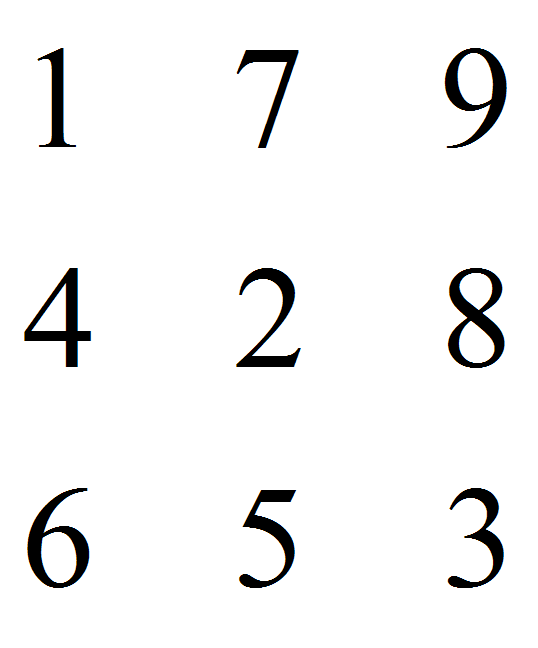
\includegraphics[width=1.552cm,height=1.87cm]{img/CMCIBasicCourse201102-img64.png}
\[
 \begin{matrix}
  1 & 7 & 9 \\
  4 & 2 & 8 \\
  6 & 5 & 3
 \end{matrix}
\]

Then we align these numbers in the ascending order. 

\ \ 1 2 3 4 5 6 7 8 9

We take the median of this sequence ($=5$) and replace the value 2 with
5.
\subsection{Morphological Image Processing}

Mathematical morphology is a powerful tool that can be used to extract
features and components from an image. It is often used to pre-process
or post-process of images to facilitate analysis. In this process a
small shape (structuring element, not necessarily square like we did in
the precious section) is translated across the image during the course
of processing. Certain mathematical logic operations are performed on
the image using the structuring element to generate the processed
image.
In this section, we first introduce dilation and erosion, two
fundamental operations in mathematical morphology. We then describe
morphological operations obtained by combining erosion and dilation. 
\subsubsection{Dilation}
Dilation is an operation that grows objects in a binary image. The
thickening is controlled by a small structuring element. In Fig. \ref{fig:img65} 
you can see the structuring element on the right and
the result after applying dilation on a rectangle.

%figure
% \begin{figure}[htbp]
% \begin{center}
% 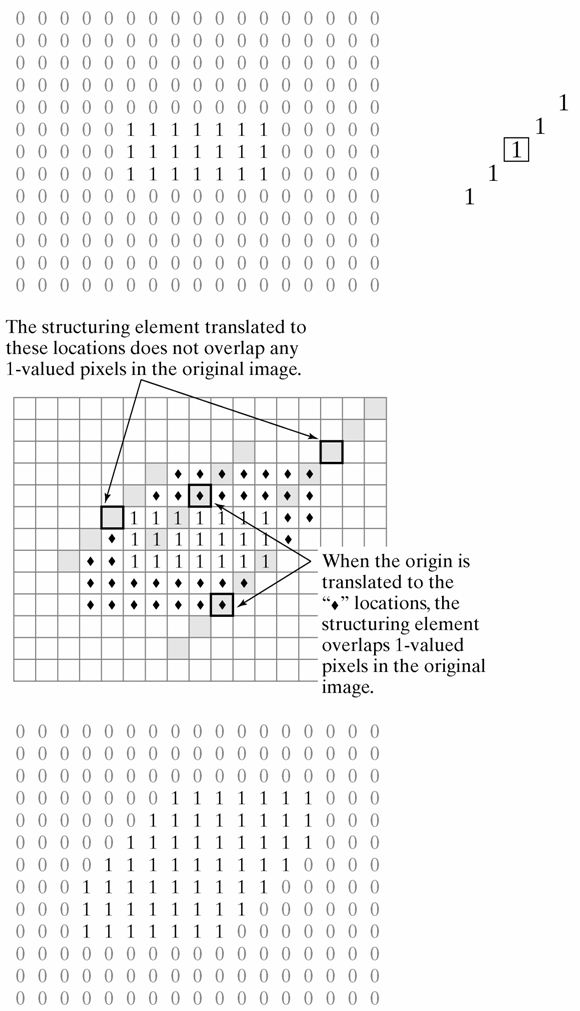
\includegraphics[width=9.222cm]{img/CMCIBasicCourse201102-img65.png}
% \caption{ Dilation (figure taken from DIP).}
% \label{fig:img65}
% \end{center}
% \end{figure}



\subsubsection{Erosion}
Erosion shrinks or thins objects in a binary image. After erosion the
only pixels that survive are those where the structuring element fits
entirely in the foreground (Fig. \ref{fig:img66}).

%figure
\begin{figure}[htbp]
\begin{center}
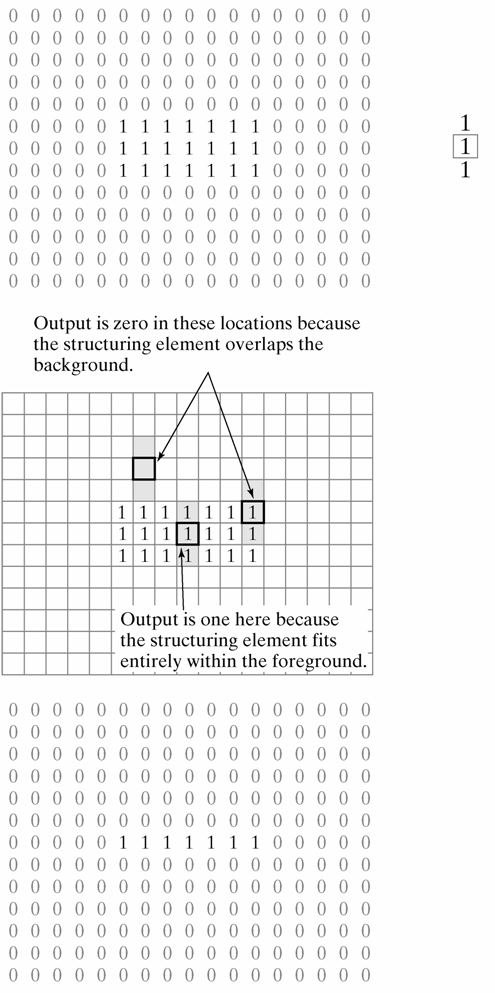
\includegraphics[width=8cm]{img/CMCIBasicCourse201102-img66.png}
\caption{ Erosion (figure taken from DIP)}
\label{fig:img66}
\end{center}
\end{figure}

In above examples structuring elements are asymmetrically shaped. In
ImageJ, structuring elements are squares so the dilation: erosion
effects are even along both axes. 

\begin{indentexercise}{1}
Load noisy-fingerprint.tif and broken-text.tif. Apply dilations or
erosions with different iterations. 

For setting iterations, do \ijmenu{[Process > Binary > Options]}. 
Binary option window opens and you can set
several parameters. "Count"
matters with setting the number of overlapping pixels between
structuring element and the object that determines output 0 or 1.
Larger count causes less degree of erosion or dilation.

%figure
\begin{figure}[htbp]
\begin{center}
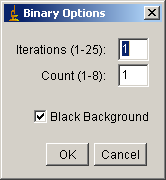
\includegraphics[width=4cm]{img/CMCIBasicCourse201102-img67.png}
\caption{ Setting Iteration.}
\label{fig:img67}
\end{center}
\end{figure}
\end{indentexercise}

\begin{quote}
From ImageJ manual: Iterations specifies the number of times erosion,
dilation, opening, and closing are performed. Count specifies the
number of adjacent background pixels necessary before a pixel is
removed from the edge of an object during erosion and the number of
adjacent foreground pixels necessary before a pixel is added to the
edge of an object during dilation. Check Black Background if the image
has white objects on a black background.
\end{quote}

\subsection{Morphological processing: Opening and Closing}

Combinations of morphological operations can be very useful in removing
many artifacts present in images. This will become very useful after
segmenting an image. The first operation we will see is opening, which
is an erosion followed by dilation. Opening smooths object contours,
breaks thin connections and removes thin protrusions. After opening,
all objects smaller than the structuring element will disappear.
Closing is a dilation followed by erosion. Closing smooths object
contours, joins narrow breaks, fills long thin gulfs and fills holes
smaller than the structuring element.

\begin{indentexercise}{1}
Load noisy-fingerprint.tif and broken-text.tif. Apply
opening and closing to the images by \ijmenu{[Process 
> Binary > Open]} and \ijmenu{[Process > Binary > Close]}. 
\end{indentexercise}


\begin{indentexercise}{2}
(Optional) Next, we do morphological processing using anisotropic structuring
element. 

Invoke \ijmenu{[Plugins > CMCICourseModules > Morphology]} and design vertical structuring element first with (1)
diameter = 3. This is simply by inputting
"3" in the Diameter field. Click tiles
to activate/deactivate positions. Click
"Apply" button to do the actual
processing. Then you could try with a larger diameter: (2) diameter =
9. Apply these two different structuring elements to dilate
noisy-finger print. Discuss the difference in outputs. 


%figure
\begin{figure}[htbp]
\begin{center}
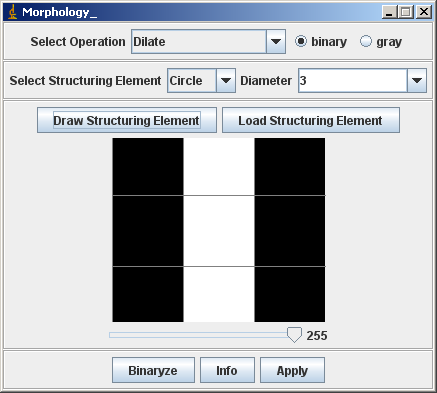
\includegraphics[width=6.5cm]{img/CMCIBasicCourse201102-img68.png}
\caption{ Morphological Image Processing dialog, to design structuring element.}
\label{fig:img68}
\end{center}
\end{figure}
\end{indentexercise}

\subsection{Minimum and Maximum}

Morphological transformation on grayscale image is very useful for
subtracting the background, such as to eliminating the shading of the
image such as shown in fig below. Opening and closing we studied above
works only with binary images. For gray scale images, one can use
Minimum (like Open) and Maximum (like Close) under [Process
Filters]. One could remove all features smaller than
the structuring element by "Minimum"
operation of gray images. In the following example we will experience
this.

\begin{indentexercise}{1}
\label{exer:removerice}
Open rice.tif. Then \ijmenu{[Process > Filters > Minimum]}. In the dialog
window, input the radius of the structuring element (structuring
element is circular). Find a radius that removes rice from the image.
Successfully removed image is the background image. Then remove the
background image from the original image. 

\textit{Note}: removal should
be based on division for brightfield images and such as: 
\[
Corrected\_Image = \frac{Specimen - Darkfield}{Brightfield - Darkfield} * 255
\]
\end{indentexercise}



\subsection{Background Subtraction}

Besides the background subtraction we studied above using Minimum and
Maximum filtering, there are special function designed for the
background subtraction (extension of morphological processing). ImageJ
has a direct background subtraction by Rolling ball algorithm \footnote{
Stanley Sternberg's article, "Biomedical Image Processing", IEEE Computer, January 1983). }
In the dialog window when you execute this operation, you will be asked for
the Rolling ball radius. This should be at least as large as
the radius of the largest object in the image that is not part of the
background.

%figure
\begin{figure}[htbp]
\begin{center}
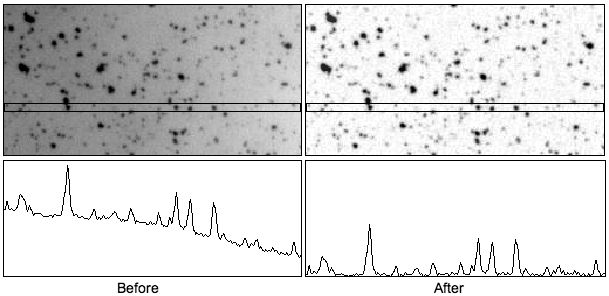
\includegraphics[width=11.875cm]{img/CMCIBasicCourse201102-img69.jpg}
\caption{ Background Subtraction (from ImageJ site).}
\label{fig:img69}
\end{center}
\end{figure}


\begin{indentexercise}{1}
Open rice.tif. Do background
subtraction by \ijmenu{[Process > Subtract > Background]}.
Change the Rolling ball radius and study the effect. Question: what
happens when the rolling ball radius is smaller?
\end{indentexercise}

More practical information on background subtraction (including
microscopy set up) is available in ImageJ
wiki\footnote{\url{http://imagejdocu.tudor.lu/imagej-documentation-wiki/how-to/how-to-correct-background-illumination-in-brightfield-microscopy}}. For flat field correction protocol, see "Optical
Microscopy Primer"
site\footnote{\url{http://micro.magnet.fsu.edu/primer/digitalimaging/imageprocessingintro.html}}.


\subsection{Other Functions: Fill holes, Skeltonize, Outline}

Frequently, after some morphological operation we need to fill the holes
in a binary image. For example, we detect the boundary of a cell and
want to obtain an object which is filled and covers the cell. In this
example we will see its effect.

\begin{indentexercise}{1}
Open \textbf{book-text.tif}. Then fill holes by \ijmenu{[Process >
Binary > Fill Holes]}. 
\end{indentexercise}

\clearpage
\subsection{Batch Processing Files}

Once you established a processing protocol, then you could create a
pipeline to process many files automatically one-by-one. Such task is
called \textit{batch processing}.
Prerequisite for using batch processing function in ImageJ is that all
files that you want to process are stored in a single folder. Another
preparation for batch processing is that you should
\textit{record} the processing command,
in the following way shown in the exercise.



\begin{indentexercise}{1}
Here, we use numbered-tiff file series as an example to do batch
processing. Open
\textbf{/sample\_images/spindle-frames/eg5\_spindle\_500016.tif}. In order to
to record the processing command, do \ijmenu{[Plugins 
Macros Recorder\ldots]}. A recorder window starts up:

%figure
\begin{figure}[htbp]
\begin{center}
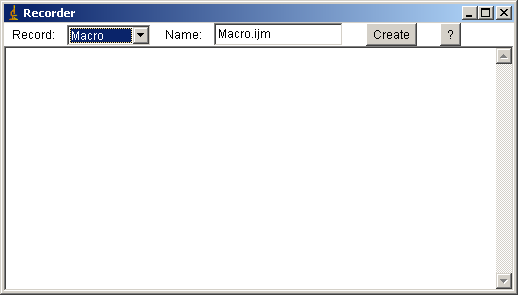
\includegraphics[width=8.678cm,height=4.942cm]{img/CMCIBasicCourse201102-img70.png}
\caption{ Macro Recorder Window}
\label{fig:img70}
\end{center}
\end{figure}


Then go back to the spindle image (activate the image window by clicking
the title bar) and then do \ijmenu{[Process > Subtract > Background]}. Just put some values in the subtract background dialog,
and click OK, and check that the image is background subtracted (Fig. \ref{fig:spindleBacksubtraction}). 


%double figure
\begin{figure}[htbp]
 \centering
 \subfloat[]{\label{fig:img71}
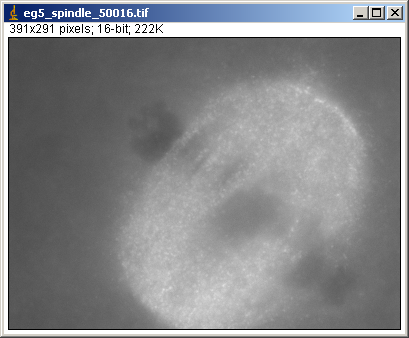
\includegraphics[height=6cm]{img/CMCIBasicCourse201102-img71.png}
}
 \subfloat[]{\label{fig:img72}
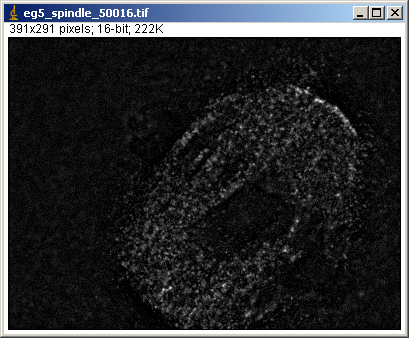
\includegraphics[height=6cm]{img/CMCIBasicCourse201102-img72.png}}
 \caption{ Spindle images (a) before and (b) after the
background subtraction.}
 \label{fig:spindleBacksubtraction}
\end{figure} 


Check the Recorder window again. You will see that a new text line is
added. This text should be like it is shown in Fig. \ref{fig:img73}.

\begin{quote}
\ilcom{run("Subtract background\ldots", "rolling=5 disable");}
\end{quote}

number after \ijmenu{rolling=} could be
various according to your input, and also other arguments might be
present after that depending on the checks you did during the Subtract
Background dialog. 
%figure
\begin{figure}[htbp]
\begin{center}
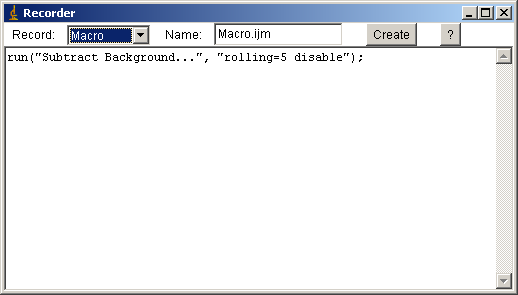
\includegraphics[width=8cm]{img/CMCIBasicCourse201102-img73.png}
\caption{ Recorder window after Subtract Background command.}
\label{fig:img73}
\end{center}
\end{figure}

Copy and paste this text command, and paste it somewhere to keep it.
Then do \ijmenu{[Process > Batch > Macro\ldots]}. This will create a new window titled
"batch Process". Paste the text
command you prepared above in the text field of this batch Process
window (Fig. \ref{fig:img74}). 

%figure
\begin{figure}[htbp]
\begin{center}
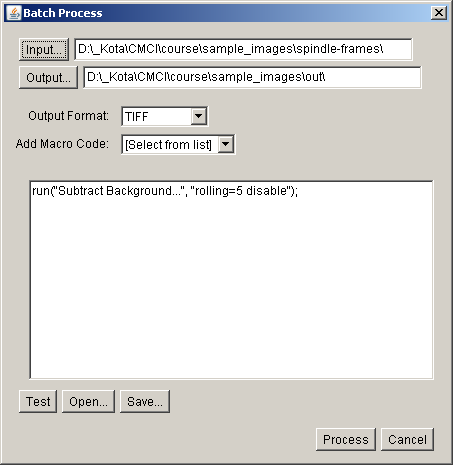
\includegraphics[width=8.881cm,height=9.116cm]{img/CMCIBasicCourse201102-img74.png}
\caption{ Batch Process window.}
\label{fig:img74}
\end{center}
\end{figure}


To set the input folder (where files to be processed are stored), click
"Input\ldots" button and select the
folder. Then set the out put folder (where processed files will be
stored, choose one that is empty), click
"Output" button and select a folder.
Check the options so that they look like above, then clicking
"Process" button will start the batch
processing of all files in the input folder. Check the images created
in the output folder to see images are actually the processed version
of input folder.
\end{indentexercise}

In above exercise, we had only one processing command, but you could add
many more text commands, which you could extract by using
"Recorder".
\subsection{Fast Fourier Transform (FFT) of Image}

FFT converts spatial-domain image data (what you are normally seeing
image) to frequency domain data. FFT is used because 
\begin{enumerate}
\item in some occasion, calculation could be done much faster in frequency domain
than in spatial domain. \textit{i.e.} convolution. 
\item Some image-processing techniques could only be done in frequency domain. 
\end{enumerate}

\begin{indentexercise}{1}
Reversibility of FFT

Open \textbf{microtubule.tif} by \ijmenu{[File > Open]}. Then apply FFT by \ijmenu{[Process > FFT > FFT]}. A new window showing frequency-domain image (2D power spectrum, log display) appears. To check that FFT is reversible, apply \ijmenu{[Process > FFT > Inverse FFT]} (Fig. \ref{fig:FFTreversibility}).

\end{indentexercise}

%triple figure
\begin{figure}[htbp]
 \centering
 \subfloat[]{\label{fig:img75}
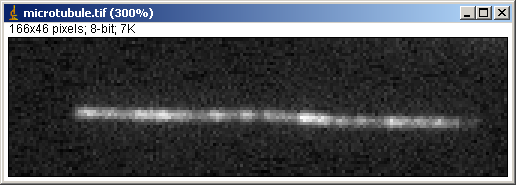
\includegraphics[width=3.889cm,height=1.393cm]{img/CMCIBasicCourse201102-img75.png}}
 \subfloat[]{\label{fig:img76}
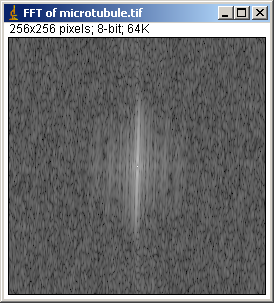
\includegraphics[width=2.447cm,height=2.706cm]{img/CMCIBasicCourse201102-img76.png}}
 \subfloat[]{\label{fig:img77}
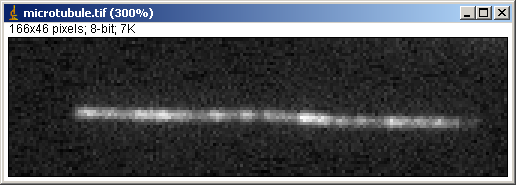
\includegraphics[width=3.889cm,height=1.393cm]{img/CMCIBasicCourse201102-img77.png}}
 \caption{ Reversibility of FFT. (a) Original, (b) FFT, (c) Inverse FFT.}
 \label{fig:FFTreversibility}
\end{figure} 

Here is an intuitive explanation of what frequency domain image is:
Orientation of patterns in spatial domain image has a clear
relationship with the resulting FFT image. We take example four images
with stripes differently oriented, vertical, diagonal (right to left or
left to right) and horizontal (Fig. \ref{fig:FFTOriginalStripesDirections})\footnote{\ To generate such stripe images for studying FFT, use macro code in Appendix \ref{app7}. }. When
these images are transformed by FFT, resulting images show high
intensity peaks (which means higher value) that reflect the direction 
of stripe pattern (Fig. \ref{fig:FFTtransformedStripesDirections}). 

%4 figures
\begin{figure}[htbp]
 \centering
 \subfloat[]{\label{fig:img78}
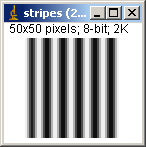
\includegraphics[width=3cm]{img/CMCIBasicCourse201102-img78.png}}
 \subfloat[]{\label{fig:img79}
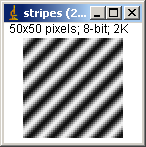
\includegraphics[width=3cm]{img/CMCIBasicCourse201102-img79.png}}
 \subfloat[]{\label{fig:img80}
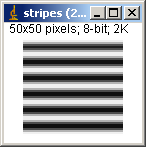
\includegraphics[width=3cm]{img/CMCIBasicCourse201102-img80.png}}
 \subfloat[]{\label{fig:img81}
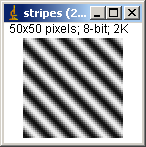
\includegraphics[width=3cm]{img/CMCIBasicCourse201102-img81.png}}
 \caption{ Original images (Spatial-domain images).}
 \label{fig:FFTOriginalStripesDirections}
\end{figure} 

%4 figures
\begin{figure}[htbp]
 \centering
 \subfloat[]{\label{fig:img82}
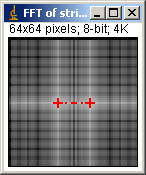
\includegraphics[width=3cm]{img/CMCIBasicCourse201102-img82.png}}
 \subfloat[]{\label{fig:img83}
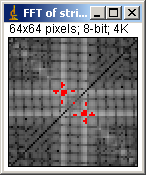
\includegraphics[width=3cm]{img/CMCIBasicCourse201102-img83.png}}
 \subfloat[]{\label{fig:img84}
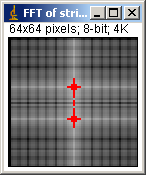
\includegraphics[width=3cm]{img/CMCIBasicCourse201102-img84.png}}
 \subfloat[]{\label{fig:img85}
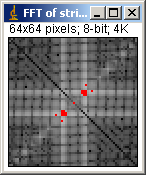
\includegraphics[width=3cm]{img/CMCIBasicCourse201102-img85.png}}
 \caption{ FFT images (Frequency-domain images). High intensity values are highlighted in red.}
 \label{fig:FFTtransformedStripesDirections}
\end{figure} 


For example, FFT image of stripes in horizontal direction (Fig. \ref{fig:img78}) shows high intensity peaks that are horizontally aligned (Fig. \ref{fig:img82}). 
Stripes in vertical direction (Fig. \ref{fig:img80}) become vertically
aligned peaks in FFT image (Fig. \ref{fig:img84}). 
In general, values in FFT image would show peaks aligned in the direction of the repetitive pattern appeared in original spatial-domain image. If the pattern appears in all direction (isotropic pattern, such as concentric rings) would then end up in circular signal in FFT image. 

Frequency of patterns in spatial-domain image also has a clear
relationship with the resulting FFT image. See spatial-domain images
shown in below. Stripe frequency decreases from left to right. In
corresponding FFT images shown in the second row, high-intensity pixels
(high-lighted in red) become closer to the center of FFT image as the
frequency of pattern in the original spatial-domain image decreases. 

%4 figures
\begin{figure}[htbp]
 \centering
 \subfloat[]{\label{fig:img86}
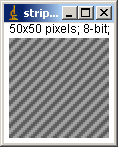
\includegraphics[width=3cm]{img/CMCIBasicCourse201102-img86.png}}
 \subfloat[]{\label{fig:img87}
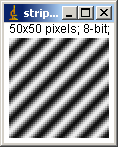
\includegraphics[width=3cm]{img/CMCIBasicCourse201102-img87.png}}
 \subfloat[]{\label{fig:img88}
\includegraphics[width=3cm]{img/CMCIBasicCourse201102-img88.png}}
 \subfloat[]{\label{fig:img89}
\includegraphics[width=3cm]{img/CMCIBasicCourse201102-img89.png}}
 \caption{ Original images (Spatial-domain images) with various frequency.}
 \label{fig:FFTOriginalStripesFrequencies}
\end{figure} 

%4 figures
\begin{figure}[htbp]
 \centering
 \subfloat[]{\label{fig:img90}
\includegraphics[width=3cm]{img/CMCIBasicCourse201102-img90.png}}
 \subfloat[]{\label{fig:img91}
\includegraphics[width=3cm]{img/CMCIBasicCourse201102-img91.png}}
 \subfloat[]{\label{fig:img92}
\includegraphics[width=3cm]{img/CMCIBasicCourse201102-img92.png}}
 \subfloat[]{\label{fig:img93}
\includegraphics[width=3cm]{img/CMCIBasicCourse201102-img93.png}}
 \caption{ FFT images (Frequency-domain images) of images with various frequency.}
 \label{fig:FFTtransformedStripesFrequencies}
\end{figure} 

Frequency-domain image is a plot with vertical frequency in vertical
axis and horizontal frequency in horizontal axis. Two axis crosses at
the centre of the image. Schematic drawing of FFT image in below shows
how FFT signal would be distributed in terms of original spatial-domain
image. 

% Unhandled or unsupported graphics:
%\includegraphics[width=9.262cm,height=9.855cm]{CMCIBasicCourse201102-img94}
%figure
% \begin{figure}[H]
% \begin{center}
% \includegraphics{eps/FFTscheme.eps}
% \caption{ Distribution of Signals in 2D Power Spectrum. Frequency of pattern increases from center towards periphery (black arrows). Direction of pattern is reflected in the alignment of signal in 2D power spectrum.}
% \label{fig:imgFFT}
% \end{center}
% \end{figure}

Signals with lower frequency, such as objects, will be placed close to
the origin (center of the 2D power spectrum image), while higher frequency signals
such as noise will be placed further from the origin. Noise in general has no spatial bias, so the signal of noise will predominantly appear in all over the peripheral region of 2D power spectrum (FFT image). 
Anisotropic patterns in original image will results in anisotropic signal in 2D power spectrum \textit{e.g.} horizontal pattern will cause horizontally aligned high intensity peaks. 

\subsection{Frequency-domain Filtering}

Filtering using FFT image (2D power spectrum) is a way of improving image quality and
also for efficient segmentation. One typical example would be noise
reduction. As we have seen in Fig. \ref{fig:imgFFT}, noise is high frequency
isotropic signal that will be in the periphery of FFT image. We
could then remove noise by simply throwing away peripheral signals in FFT
image to reduce noise. 

\begin{indentexercise}{1} Removing noise using FFT image. 

Open \textbf{microtubule.tif} by \ijmenu{[File > Open]}. Then apply FFT
by \ijmenu{[Process > FFT > FFT]}. A new
window showing microtubule converted to a frequency-domain image (2D power spectrum) appears. Make
a rectangular ROI covering vertical streak at the center of the FFT
image, and then \ijmenu{[Image > Clear > Outside]} to
convert peripheral signals to 0 (black. If Clear Outside produced white
periphery, check \ijmenu{[Edit > Options > Colors]} to
see if the background color is black). \ijmenu{[Process 
> FFT > Invert FFT]} to see the spatial-domain image after
filtering.
\end{indentexercise}

Similar to this exercise, we could separate a spatial domain image to high-frequency part
and low-frequency part to isolate two overlapping signals to each, such as shown
with an example below.
 
Adding high-frequency (Fig. \ref{fig:img95}) and low-frequency (Fig. \ref{fig:img96}) stripe images 
results in an overlapped image of two frequencies (Fig. \ref{fig:img97}). This image math could be done
easily using \ijmenu{[Process > Image Math]} . It is not easy
to isolate each of two original images from this overlapped image by spatial domain filtering, but
it could be done in a pretty simple way if you FFT Fig. \ref{fig:img97} image and use the frequency-domain image (Fig. \ref{fig:img99}). 
FFT image could be separated to two images, one from the center (called "low-pass", Fig. \ref{fig:img100}) 
and the other from peripheral (called "high-pass",  Fig. \ref{fig:img101}). 
\ijmenu{[Process > FFT > Invert FFT]} of each FFT image would result low-frequency stripe image  (Fig. \ref{fig:img103}) and
high-frequency stripe image (Fig. \ref{fig:img105}).

%triple figure
\begin{figure}[htbp]
 \centering
 \subfloat[]{\label{fig:img95}
\includegraphics[width=3cm]{img/CMCIBasicCourse201102-img95.png}
}
 \subfloat[]{\label{fig:img96}
\includegraphics[width=3cm]{img/CMCIBasicCourse201102-img96.png}
}
 \subfloat[]{\label{fig:img97}
\includegraphics[width=3cm]{img/CMCIBasicCourse201102-img97.png}
}
 \caption{ Images of (a) high frequency pattern, (b) low frequency pattern, (c) a and b combined.}
 \label{fig:patternCombining}
\end{figure} 


%triple figure
\begin{figure}[htbp]
 \centering
 \subfloat[]{\label{fig:img99}
\includegraphics[width=3cm]{img/CMCIBasicCourse201102-img99.png}
}
 \subfloat[]{\label{fig:img100}
\includegraphics[width=3cm]{img/CMCIBasicCourse201102-img100.png}
}
 \subfloat[]{\label{fig:img101}
\includegraphics[width=3cm]{img/CMCIBasicCourse201102-img101.png}
}
 \caption{ (a) FFT image (2D power spectrum) of Fig. \ref{fig:img97} could be separated to (b) low frequency part near the origin and (c) high frequency part in the periphery.}
 \label{fig:2DpowerSeparation}
\end{figure} 


%double figure
\begin{figure}[htbp]
 \centering
 \subfloat[]{\label{fig:img102}
\includegraphics[width=3cm]{img/CMCIBasicCourse201102-img102.png}
}
 \subfloat[]{\label{fig:img103}
\includegraphics[width=3cm]{img/CMCIBasicCourse201102-img103.png}
}
 \caption{ (a) Lower frequency part could then be invert-FFT to visualize (b) only the low-frequency pattern.}
 \label{fig:invertToGetLowFrequencyImage}
\end{figure} 

%double figure
\begin{figure}[htbp]
 \centering
 \subfloat[]{\label{fig:img104}
\includegraphics[width=3cm]{img/CMCIBasicCourse201102-img104.png}
}
 \subfloat[]{\label{fig:img105}
\includegraphics[width=3cm]{img/CMCIBasicCourse201102-img105.png}
}
 \caption{ (a) Higher frequency part could then be invert-FFT to visualize (b) only the high-frequency pattern.}
 \label{fig:invertToGetHighFrequencyImage}
\end{figure} 


Above was an example of low-pass filtering (for isolating low frequency
stripes) and high-pass filtering (for isolating high frequency signal).
We could utilize more complex filters to isolated more specific
frequency signals. Such filter is called \textit{band pass
filter}. Band pass filtering is
available in \ijmenu{[Process > FFT > Band Pass Filter\ldots]}. 


\subsection{ASSIGNMENTS}

\textbf{\sffamily
Assignment 1-3-1: Convolution and Kernels
}

\begin{enumerate}
\item Design your own kernel, apply it to an image of your choice and
discuss what it does. 

\item Gaussian kernel: Open the Gaussian kernels (in sample image folder,
Gss5x5.txt, Gss7x7.txt and Gss15x15.txt) by \ijmenu{[File >
Import > Text Image]}. Then try getting the
line profile of 2D Gaussian, crossing the peak of the curve. The line
profile across the 2D Gaussian should be 1-D Gaussian curve. Save the
resulting graphs as image files. 

\item Visualize the Gaussian kernel using the "surface
plot" \ijmenu{[Analyze > Surface Plots{\dots]}}.
\end{enumerate}

